%%%%%%%%%%%%%%%%%%%%%%%%%%%%%%%%%%%%%%%%%
% Revista Difu100cia
%%%%%%%%%%%%%%%%%%%%%%%%%%%%%%%%%%%%%%%%%
\documentclass[12pt]{difu100cia} % clase difu100cia

%----------------------------------------------------------------------------------------
%	PAQUETES ADICIONALES
%----------------------------------------------------------------------------------------



%----------------------------------------------------------------------------------------
%	DECLARACION DE COMANDOS
%----------------------------------------------------------------------------------------




%----------------------------------------------------------------------------------------
%	INFORMACION DEL ARTICULO
%----------------------------------------------------------------------------------------

\title{Acciones que promueven la inclusión del marketing digital en MIPYMES de Xicotepec} % Titulo del articulo en ingles
% Autores
\author[1]{\authorstyle{Quiroz Ramírez-Isabel}}
\author[1]{\authorstyle{Cruz Suárez- Silvia Denisse}\thanks{Autor de correspondencia}}
\author[1]{\authorstyle{Galindo González-Oscar}}
\author[1]{\authorstyle{Amador Mendoza- Evelin1}}
\author[1]{\authorstyle{Velázquez Vargas-José Rubén}}
\author[1]{\authorstyle{Tolentino Castillo- Guadalupe}}
%\author[2]{\authorstyle{Juán Perez}}
\affil[1]{\institution{Universidad Tecnológica de Xicotepec de Juárez (UTXJ), Área Económico-Administrativa, \authorcr Cuerpo Académico. Desarrollo empresarial, \authorcr Av. Universidad Tecnológica No. 1000, Col. Tierra Negra, Xicotepec de Juárez, Puebla. C.P. 73080. \authorcr quirozisabel1983@hotmail.com,\{(isabel.quiroz, silvia.cruz, oscar.galindog, evelin.amador, ruben.velazquez, guadalupe.tolentino\}@utxicotepec.edu.mx }}
%\affil[2]{\institution{Universidad Tecnológica de Xicotepec de Juárez}}

%----------------------------------------------------------------------------------------
%   Fecha de publicación
%----------------------------------------------------------------------------------------

\publishrange{Mayo - Agosto 2022}
\volume{13}
\num{2}
\published{12 de agosto de 2022}

%----------------------------------------------------------------------------------------

\begin{document}

\selectlanguage{spanish} % selecciona espanol como idioma
%\selectlanguage{english} % Selecciona ingles como idioma
\thispagestyle{firstpage} % Aplica el estilo en la primera pagina sin cabeceras y pie de pagina
\maketitle % Imprime el titulo
\pagestyle{fancy}

%----------------------------------------------------------------------------------------
%	RESUMEN
%----------------------------------------------------------------------------------------

\begin{abstract}[english]
This research work aims to analyze the different activities that allow the implementation of digital marketing in MSMEs in Xicotepec. It is vital for companies in general to develop strategies that strengthen their capacity and the continuous search for competitive advantages, making it essential to research and implement improvements in all areas. 
As a proposal on this occasion, we present research that aims to articulate different mechanisms that allow MSMEs in Xicotepec the knowledge, management, and inclusion of digital marketing in their operations since because of the pandemic situation we are going through, was caused these introduced in an untimely manner the sale of their products and services with the use of digital tools; using mainly WhatsApp and Facebook, as means of advertising and distribution channel for their products, while some others implemented only the home service.
Derived from the above, a solid economic recession was generated in Xicotepec. It is now essential to identify, define and implement different strategies that allow the economic momentum in the region to contribute to the survival and promotion of MSMEs with the help of digital marketing.
For all the above described, the importance of this research is justified by pointing to the use of digital marketing to contribute to the economic recovery of MSMEs in Xicotepec de Juárez, which according to data from the 2019 Economic Census, the sectors that concentrated the most significant number of economic units were: retail trade (1,880 units), manufacturing industries (639 units) and other services except government activities (617 units).

\end{abstract}

\keywords[english]{ Digital marketing, MSMEs, digital tools}

\begin{abstract}[spanish]
El presente trabajo de investigación tiene como finalidad analizar las diferentes actividades que permitan la implementación del marketing digital en las MIPYMES de Xicotepec. Es de vital importancia para las empresas en general el desarrollo de estrategias que promuevan el fortalecimiento de su capacidad y la búsqueda continua de ventajas competitivas, mismas que hacen primordial la investigación e implementación de mejoras en todas las áreas. 
Como propuesta se presenta esta investigación que apunta a la articulación de diferentes mecanismos que permitan a las MIPYMES de Xicotepec adquirir el conocimiento, manejo e inclusión del marketing digital en sus operaciones, ya que a consecuencia de la pandemia generada por el virus COVID 19 que estamos atravesando, se ocasiono que estas entidades económicas introdujeran de manera intempestiva la venta de sus productos y servicios con la utilización de herramientas digitales; utilizando principalmente WhatsApp y Facebook, como medios de publicidad y canal de distribución para sus productos, mientras que algunos otros implementaron solo el servicio a domicilio.
Derivado de lo anterior se generó una fuerte contracción económica en Xicotepec por lo que es primordial  identificar, definir y aplicar diferentes estrategias que permitan el impulso económico en la región coadyuvando a la supervivencia e impulso de las MIPYMES, mediante la ayuda del marketing digital.
Por todo lo anteriormente descrito, se justifica la relevancia de esta investigación apuntando a la utilización del marketing digital para contribuir a la recuperación económica de las MIPYMES de Xicotepec de Juárez, Puebla; que según los datos del Censo Económico 2019, los sectores que concentraron mayor cantidad de unidades económicas fueron: comercio al por menor (1,880 unidades), industrias manufactureras (639 unidades) y otros servicios exceptuando actividades gubernamentales (617 unidades).
\end{abstract}

\keywords[spanish]{Marketing digital, MIPYMES, herramientas digitales}

%----------------------------------------------------------------------------------------
%	ARTICULO
%----------------------------------------------------------------------------------------

\section{Introducción}
Es importante definir que como estrategia central objeto de esta investigación se abordará principalmente el marketing digital, mismo que se ha convertido en una herramienta para el comercio.
Según datos del INEGI el 99.8\% de las unidades de negocio, pertenecen al segmento de micro, pequeña y mediana empresa, con más de 4.1 millones de empresas que aportan el 42\% del Producto Interno Bruto. (PIB).
En el año 2020 más de un millón de empresas tuvieron que cerrar sus puertas. Cabe mencionar que durante este período también se establecieron 619,443 nuevas empresas.
El 30 de enero del 2020, la Organización Mundial de la Salud (OMS), marcó el inicio de una emergencia de salud pública de preocupación internacional, considerada ahora pandemia, ocasionada por el incremento de casos causados por el virus COVID-19, cuyos contagios se extendieron en varios países del mundo.
Es menester de este trabajo; presentar los resultados del estudio realizado y poder a través de ellos proponer las líneas de acción a seguir para la adquisición e implementación de mecanismos necesarios que permitirán a resumidas cuentas, el posicionamiento de la actividad económica de las MIPYMES: y que al mismo tiempo generará la reactivación económica de Xicotepec de Juárez, Puebla; minimizando así los efectos de la Pandemia causada por el virus SARS COV 2.


\section{Marco teórico}

Al hablar de marketing podemos encontrar diferentes definiciones, por ejemplo: Philip Kotler la define como “un proceso social y administrativo mediante el cual grupos e individuos obtienen lo que necesitan y desean a través de generar, ofrecer e intercambiar productos de valor con sus semejantes” .
Por otra parte, para Stanton, Et. al, indican que: ["El marketing es un sistema total de actividades de negocios ideado para planear productos satisfactores de necesidades, asignarles precios, promover y distribuirlos a los mercados meta, a fin de lograr los objetivos de la organización".]
Según el libro de la Guerra del marketing, para John A. Howard, de la Universidad de Columbia, {"el marketing es el proceso de: 1) Identificar las necesidades del consumidor, 2) conceptualizar tales necesidades en función de la capacidad de la empresa para producir, 3) comunicar dicha conceptualización a quienes tienen la capacidad de toma de decisiones en la empresa. 4) conceptualizar la producción obtenida en función de las necesidades previamente identificadas del consumidor y 5) comunicar dicha conceptualización al consumidor".}
De las contribuciones más importantes que ha realizado Kotler es la ampliación del concepto de marketing, estableciendo que es una nueva forma de comunicación e intercambio con los clientes, no solo para comercializar sino también para forjar experiencias únicas. Es decir, que el marketing puede utilizarse para influenciar el comportamiento de diversos sectores de la población al ser un proceso social y administrativo. De esta manera, los consumidores obtienen lo que desean a través de ofertas e intercambios de productos de valor y como vendedor creas un lazo de fidelidad con éstos.  
El marketing a través del tiempo ha evolucionado dando como resultado varias transformaciones en pro de la forma de vender los productos y servicios de las empresas, posicionamiento de las marcas, fidelización de los clientes y actualmente hacer llegar más rápido esta información de las empresas a sus clientes reales y potenciales en satisfacción de las necesidades de estos últimos.
El marketing digital se desarrolla en cuatro eras las cuales son:
Marketing 1.0: Es el marketing que la mayoría de las empresas realiza y cuya primicia era enfocarse en la inversión para el desarrollo del producto. 
Marketing 2.0: A diferencia del anterior, este tipo de marketing ya no solo busca vender calidad, sino que además comienzan a entender las necesidades y hábitos de sus clientes, con el objetivo de crear nuevos productos y servicios basándose en sus comportamientos, pues ahora es el consumidor quien define el valor del producto. 
Marketing 3.0: Se basa completamente en comprender y conocer al cliente más allá de querer venderles un producto o servicio. En este estado las empresas se diferencian entre sí por sus valores. 
Marketing 4.0: La cuarta etapa del marketing hace hincapié a la era digital y la interconectividad con las nuevas tecnologías que actualmente son de suma importancia para los mercadólogos y la sociedad. Por lo que, es una transición de lo tradicional a lo digital. A su vez, establece nuevas métricas para llegar más rápido a nuevos mercados. Su objetivo es la confianza y fidelización del cliente (Cousillas, 2018).
Gracias a Tim Berner-Lee, creador del sistema de transmisión de datos que se extendió de manera mundial y lo bautizó como la “Word Wide Web”  (Velazco, 2015), el día de hoy millones de usuarios pueden crear sitios que les pueden abrir puertas y aprovechar los espacios para hacer llegar su mensaje más allá del alcance que ofrecen los medios tradicionales. 
El marketing digital es una nueva forma comercial que lleva a cabo la empresa, utilizando la telemática y que permite a sus clientes o clientes potenciales conseguir: efectuar una consulta de un producto y/o seleccionar o adquirir la oferta existente en un momento, de un determinado producto. 
Hoy en día gracias a las redes sociales como Facebook, Twitter, tiktok, entre otros, los comerciantes pueden hacer llegar su publicidad de una manera más fácil, rápida, económica, y sobre todo teniendo el dominio de la información que proporcionan a sus clientes, contando con la ventaja adicional de poder contactarse con sus posibles clientes sin la necesidad de estar en el mismo espacio físico. 
Por lo anterior entenderemos al marketing digital como: los procesos y gestiones necesarias para conocer las necesidades del cliente, transformándolas en conceptos de servicios o productos que ofrecen las empresas a sus consumidores potenciales a través de la difusión de los conceptos de servicios o productos mediante los diferentes medios digitales existentes. Es por ello que se hace de primordial importancia implementar algunas acciones que coadyuven a que las MIPYMES de Xicotepec de Juárez, Puebla; hagan uso correcto del marketing digital para el incremento de su competitividad.

\section{Descripción del modelo}

El modelo que se utiliza para la presente investigación es de tipo cuantitativo, el cual permitirá recolectar datos basados en la opinión de empresarios sobre la implementación del uso del marketing digital y posteriormente será procesada en valores numéricos para la toma de decisiones. 

Respecto al instrumento será aplicado en la zona principal de Xicotepec, con la finalidad de identificar y definir acciones que permitan el impulso económico de las MIPYMES, a través de la inclusión del marketing digital.

Respecto a la identificación de empresas que fueron parte del muestreo, se utilizó la base de datos obtenida en el DENUE (Directorio Estadístico Nacional de Unidades Económicas), que depende del Instituto Nacional de Estadística y Geografía (INEGI). Señalando que se utilizó una clasificación de empresas a las que se les censó, entre ellas fueron dedicadas a: servicios al por mayor, comercio al por menor, servicios de esparcimiento, culturales, deportivos y otros servicios de alojamiento temporal, así como de preparación de alimentos y bebidas.      
\end{figure}

\section{Descripción de la metodología}
Primera parte:

\begin{enumerate}
  \item Preliminares

\begin{itemize}
    \item Cómo primera actividad se diseñó un instrumento de recolección de datos, mediante un formulario de google forms, el cual contempló 12 reactivos entre los cuales se cuestionó si las micro, pequeñas y medianas empresas utilizan medios electrónicos o algunas apps para dar a conocer sus productos y servicios, así como si el promocionarse en redes sociales ha aumentado las ventas de sus productos en estos últimos periodos, cabe señalar que dicho cuestionario fue aplicado a una muestra representativa de 339 empresas, resultado de una población de 2,858 empresas registradas en DENUE 2022, como se muestra en la figura 1, utilizando un nivel de confianza del 95%.

\begin{figure}[!ht]
	\centering
	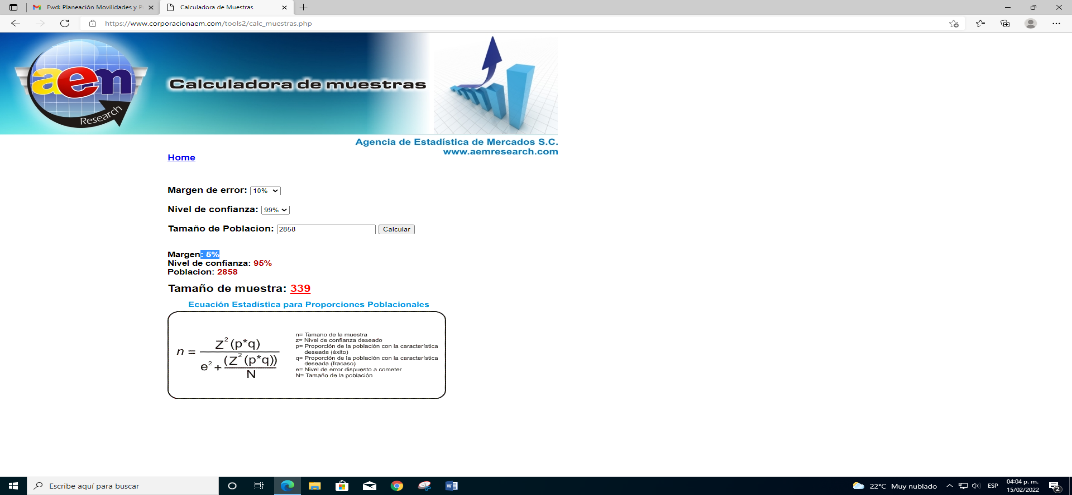
\includegraphics[width=\linewidth]{Figura 1.png}
	\caption{Muestra representativa del censo}
	
  \item Posteriormente se procedió a la aplicación del instrumentó de recolección de datos, el cual fue aplicado mediante dispositivos móviles por parte de 3 estudiantes de la carrera de T.S.U. en Administración, Área Capital Humano de la Universidad Tecnológica de Xicotepec de Juárez, quienes recibieron capacitación para la aplicación del muestreo en las empresas que corresponden de acuerdo con el giro y actividad señalada anteriormente.
  
  \item  Proceso de información: una vez que los datos fueron recolectados y procesados, se procedió al análisis e interpretación de información, la cual sirvió para identificar las condiciones y características de las MIPYMES, con relación a la inclusión del marketing digital de los negocios del municipio de Xicotepec de Juárez, Puebla.  
\end{enumerate}

\section{Resultados}

Una vez que se realizó la recolección de datos mediante la herramienta, se obtuvieron los siguientes resultados: 
\begin{figure}[!htb]
	\centering
	\includegraphics[width=\linewidth]{Figur 2.png}
	\caption{Del conocimiento de los beneficios del marketing digital}
	

En la figura 2, se puede observar que en la pregunta 1, “¿Conoce usted los beneficios del Marketing para las PYMES?” La respuesta más seleccionada por la muestra del universo de este proyecto es “Sí” con un 76,7% y la respuesta menos seleccionada es “No “con un 23.3%, por tanto, la mayoría de las personas conoce los beneficios del Marketing en las PYMES.

\begin{figure}[!htb]
	\centering
	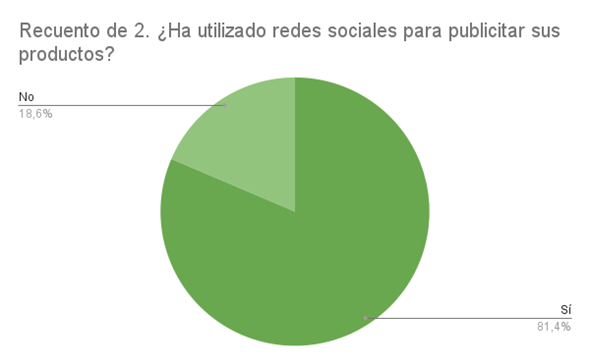
\includegraphics[width=\linewidth]{Figura 3.png}
	\caption{Utilización de redes sociales}
	
Se puede observar en la figura 3, de la pregunta: “¿Ha utilizado redes sociales para publicitar sus productos?” que la respuesta más seleccionada es “Sí” con un 81.4\% y la respuesta menos seleccionada es “No” con un 18.6\%, por tanto, la mayoría de las personas ha utilizado las redes sociales para publicitar sus productos.

\begin{figure}[!htb]
	\centering
	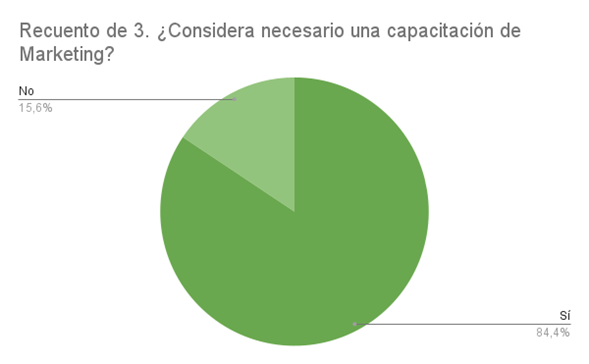
\includegraphics[width=\linewidth]{Figura 4.png}
	\caption{Necesidad de capacitación en Marketing}
	
	
En la figura 4, se identifica que a la pregunta “¿Considera necesario una capacitación de Marketing?” la respuesta más seleccionada es “Sí” con un 84.4\% y la respuesta menos seleccionada es “No” con un 15.6\%, por lo tanto, la mayoría de las personas considera necesario una capacitación de Marketing.

\begin{figure}[!htb]
	\centering
	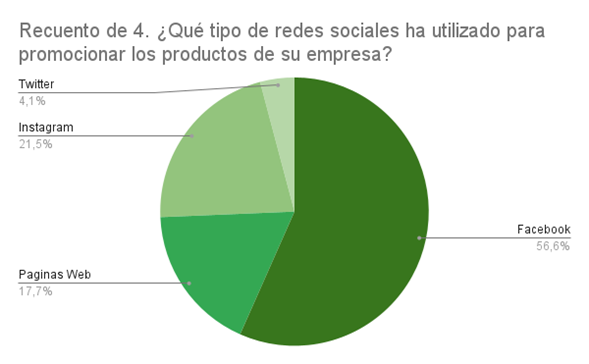
\includegraphics[width=\linewidth]{Figura 5.png}
	\caption{Tipo de redes sociales que se utilizan para promocionar los productos.}
	
	
Respecto a la pregunta 4, “¿Qué tipo de redes sociales ha utilizado para promocionar los productos de su empresa?  Se puede observar que la mayor parte de la población encuestada utiliza el “Facebook” para promocionar sus empresas, obteniendo un 56.6\% del total de la muestra, “Instagram” obtuvo un 21.5\%, “Páginas Web” un 17.7\%y la respuesta menos seleccionada es “Twitter” con un 4.1\%.

\begin{figure}[!htb]
	\centering
	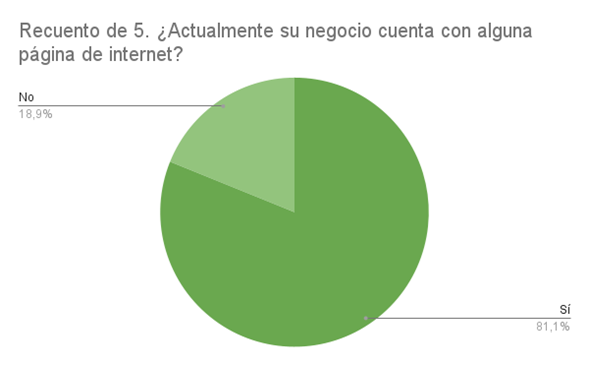
\includegraphics[width=\linewidth]{Figura 6.png}
	\caption{Tipo de redes sociales que se utilizan para promocionar los productos.}
	
	
En la figura 6, los resultados que se pueden observar como respuesta a la pregunta “¿Actualmente su negocio cuenta con alguna página de internet? La respuesta más seleccionada por la muestra es “Sí” con un 81.1\% y la respuesta menos seleccionada es “No” con un 18.9\%, por tanto, la mayoría de las personas tiene una página de internet para su negocio.

\begin{figure}[!htb]
	\centering
	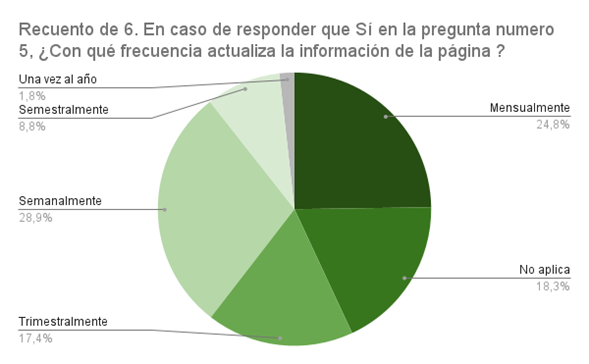
\includegraphics[width=\linewidth]{Figura 7.png}
	\caption{Frecuencia de actualización de páginas web}
	
	
Los resultados que se pueden observar en la figura 7, a “En caso de responder que Sí en la pregunta número 5, ¿Con qué frecuencia actualiza la información de la página?” La respuesta más seleccionada por la muestra es “semanalmente” con un 28.9\%, “Mensualmente” con un 24.8\%, “No aplica” con un 18.3\%, “Trimestralmente” con un 17.4\%, “Semestralmente” con 8.8\%   y la respuesta menos seleccionada es “Una vez al año” con un 1.8\%, por tanto, la mayoría de las personas actualiza la información de su página Web cada semana.

\begin{figure}[!htb]
	\centering
	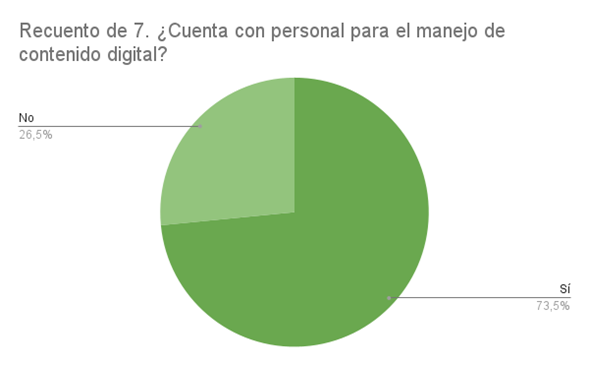
\includegraphics[width=\linewidth]{Figura 8.png}
	\caption{Existencia de personas enfocadas al manejo del contenido digital}
	
	
En la figura 8, que hace referencia a la pregunta” ¿Cuenta con personal para el manejo de contenido digital?” La respuesta más seleccionada es “Sí” con un 73.5\% y la respuesta menos seleccionada es “No” con un 26.5\%, por tanto, la mayoría de las personas cuenta con personal para el manejo de su contenido digital.

\begin{figure}[!htb]
	\centering
	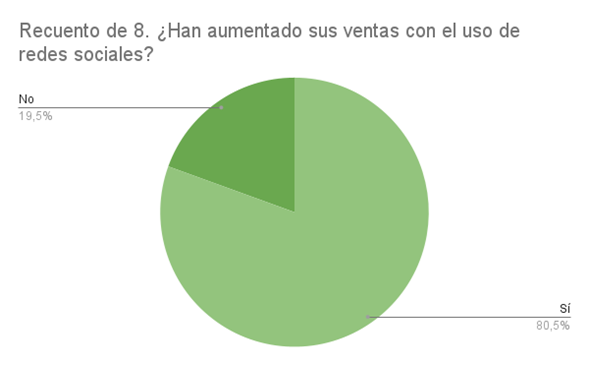
\includegraphics[width=\linewidth]{Figura 9.png}
	\caption{Incremento en ventas a causa del uso de redes sociales.}


En la figura 9, se puede observar respecto a la pregunta “¿Han aumentado sus ventas con el uso de redes sociales?” La respuesta más seleccionada por la muestra es “Sí” con un 80.5\% y la respuesta menos seleccionada es “No” con un 19.5\%, por tanto, la mayoría de las personas considera que han aumentado sus ventas con el uso de las redes sociales.

\begin{figure}[!htb]
	\centering
	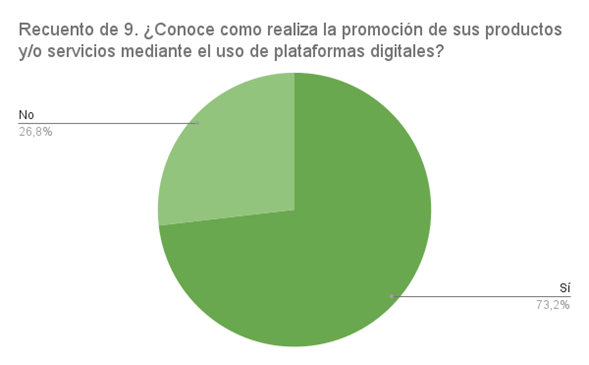
\includegraphics[width=\linewidth]{Figura 10.png}
	\caption{Manejo de plataformas de redes sociales.}
	
	
En la figura 10, en relación con la pregunta: “¿Conoce cómo realiza la promoción de sus productos y/o servicios mediante el uso de plataformas digitales?” La respuesta más seleccionada por la muestra es “Sí” con un 73.2\% y la respuesta menos seleccionada es “No” con un 26.8\%, por tanto, la mayoría de las personas conoce cómo se realiza la promoción de productos o servicios con el uso de las redes sociales.	

\begin{figure}[!htb]
	\centering
	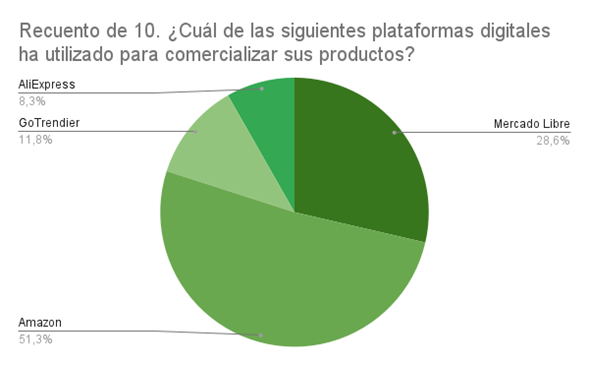
\includegraphics[width=\linewidth]{Figura 11.png}
	\caption{Que plataforma utiliza para comercializar su producto.}
	
Se observa en la figura 11, referente a la pregunta: “¿Cuál de las siguientes plataformas digitales ha utilizado para comercializar sus productos?” La respuesta más seleccionada por la muestra es “Amazon” con un 51.3, GoTrendier con un 11.8\%, “Mercado Libre” con un 28.6\%y la respuesta menos seleccionada es “AliExpress” con un 8.3\%, por tanto, la mayoría de las personas comercializa sus productos a través de Amazon.

\begin{figure}[!htb]
	\centering
	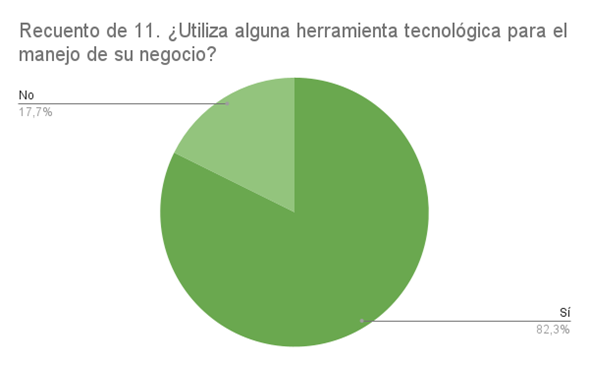
\includegraphics[width=\linewidth]{Figura 12.png}
	\caption{Del uso de herramientas para la comercialización de productos.}
	

Los resultados que se observan en la figura 12, en relación con la pregunta: “¿Utiliza alguna herramienta tecnológica para el manejo de su negocio?” La respuesta más seleccionada por la muestra es “Sí” con un 82.3\% y la respuesta menos seleccionada es “No” con un 17.7\%, por tanto, la mayoría de las personas utiliza alguna herramienta tecnológica para el manejo de su negocio.

\begin{figure}[!htb]
	\centering
	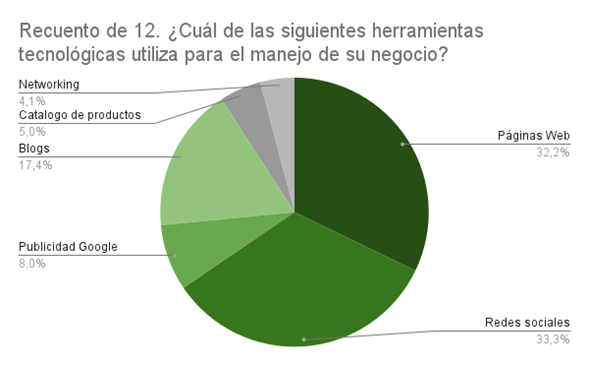
\includegraphics[width=\linewidth]{Figura 13.png}
	\caption{Herramienta tecnológica más usada para el crecimiento del negocio.}
	
	
En la figura 13 se identifican los resultados a la pregunta 12, “¿Cuál de las siguientes herramientas tecnológicas utiliza para el manejo de su negocio?” donde la respuesta más seleccionada por la muestra del universo de este proyecto es “Redes sociales” con un 33.3\%, [ “Páginas Web” con un 32.2\%, “Blogs” con un 17.4\%, “Publicidad en Google” con un 8\%, “Catálogo de productos” con un 5\% y la respuesta menos seleccionada es “Networking” con un 4.1\%, por tanto, la mayoría de las personas utiliza alguna herramienta tecnológica para el manejo de su negocio.]


\section{Análisis de los resultados}

De acuerdo a los resultados obtenidos en la investigación realizada a la muestra de MIPYMES de Xicotepec de Juárez, Puebla; en el periodo mayo – agosto de 2022, resalta que la mayoría de las personas encuestadas refieren conocer los beneficios del marketing digital, se destaca también el uso de las redes sociales para realizar la publicidad de sus productos y servicios, principalmente haciendo uso de Facebook; el 81.1\% de los negocios encuestados cuentan con página web y el 28.9\% actualiza su información cada semana. Otro aspecto identificado es que el 82.3\% de los negocios hace uso de herramientas digitales para apoyar sus operaciones, y esto ha generado que las MIPYMES encuestadas tengan la percepción de que sus ventas incrementaron debido al uso de las redes sociales donde se han promocionado; puesto que él 51.3\% realizan sus ventas por medio de Amazon, lo cual indica que se está iniciando la transición al comercio electrónico. Por otro lado, se identifica que un 73.5\% de los negocios encuestados, cuentan con personal encargado del manejo de su contenido digital, sin embargo un 84.4\% de los negocios que brindaron información, refieren requerir capacitación en marketing digital, lo cual permitiría ampliar la posibilidades de desarrollo al incluir estrategias innovadoras de promoción y publicidad digital, buscando incursionar a nuevos segmentos de mercado e incluso modificar el modelo de negocio y así poder competir en el mercado y lograr un óptimo desarrollo.


\section{Comentarios finales}

En diversas ocasiones hemos escuchado decir que se necesitan inversiones muy fuertes para poder hacer mercadotecnia digital, que la publicidad en Internet es solo para las grandes empresas, o que se necesita un equipo especializado como un diseñador o ingeniero. En realidad, la desinformación ha sido la mayor barrera para poder hacer mercadotecnia digital o para comenzar a invertir en publicidad en medios digitales.

La inversión en mercadotecnia digital para los negocios es fundamental, la implementación de acciones que permitan el posicionamiento de las marcas y/o productos en la mente del consumidor, nos permitirá proyectar un buen futuro y buscar el mayor volumen de venta de los productos que genera cualquier tipo de negocio.

La era digital nos a alcanzando incluso rebasado, un gran porcentaje de la población tiene acceso a un dispositivo móvil que nos permite estar conectados a internet y tener acceso a redes sociales, mismas que pueden ser utilizadas como trampolín para el incremento de ingresos a los diferentes negocios, solo hace falta capacitar a los interesados en el uso de estas.


%----------------------------------------------------------------------------------------
%	REFERENCIAS
%----------------------------------------------------------------------------------------

% Las referencias se deben de agregar en el archivo referencias.bib en formato bib. 

\printbibliography

%----------------------------------------------------------------------------------------

\end{document}
